\documentclass[11pt,a4paper]{article}

% ── Packages ──────────────────────────────────────────────────────────
\usepackage[utf8]{inputenc}
\usepackage[T1]{fontenc}
\usepackage{lmodern}
\usepackage[margin=1in]{geometry}
\usepackage{amsmath,amssymb,amsthm}
\usepackage{graphicx}
\usepackage{booktabs}
\usepackage{tabularx}
\usepackage{array}
\usepackage{enumitem}
\usepackage{hyperref}
\usepackage{cleveref}
\usepackage{xcolor}
\usepackage{tikz}
\usetikzlibrary{shapes.geometric,arrows.meta,positioning,fit,calc,backgrounds}
\usepackage{natbib}
\usepackage{microtype}
\usepackage{setspace}
\usepackage{fancyhdr}
\usepackage{titlesec}
\usepackage{tcolorbox}
\usepackage{caption}

% ── Colors ────────────────────────────────────────────────────────────
\definecolor{darkblue}{RGB}{0,51,102}
\definecolor{accentteal}{RGB}{1,105,111}
\definecolor{lightgray}{RGB}{245,245,245}
\definecolor{midgray}{RGB}{120,120,120}

% ── Hyperref config ───────────────────────────────────────────────────
\hypersetup{
  colorlinks=true,
  linkcolor=darkblue,
  citecolor=accentteal,
  urlcolor=accentteal,
  pdftitle={Can Is Not May: Authority Models for Governable AI Agents},
  pdfauthor={},
}

% ── Header/footer ─────────────────────────────────────────────────────
\pagestyle{fancy}
\fancyhf{}
\renewcommand{\headrulewidth}{0.4pt}
\fancyhead[L]{\small\textit{Can Is Not May}}
\fancyhead[R]{\small\thepage}

% ── Section formatting ────────────────────────────────────────────────
\titleformat{\section}{\Large\bfseries\color{darkblue}}{\thesection}{1em}{}
\titleformat{\subsection}{\large\bfseries\color{darkblue!80}}{\thesubsection}{1em}{}
\titleformat{\subsubsection}{\normalsize\bfseries\color{darkblue!60}}{\thesubsubsection}{1em}{}

% ── Theorem environments ──────────────────────────────────────────────
\newtheorem{definition}{Definition}[section]
\newtheorem{proposition}{Proposition}[section]

% ── Custom commands ───────────────────────────────────────────────────
\newcommand{\May}{\textsc{May}}
\newcommand{\Can}{\textsc{Can}}
\newcommand{\authoritymodel}{\textit{authority model}}

% ── Spacing ───────────────────────────────────────────────────────────
\setstretch{1.15}

% ══════════════════════════════════════════════════════════════════════
\begin{document}

% ── Title ─────────────────────────────────────────────────────────────
\begin{center}
  {\LARGE\bfseries\color{darkblue} Can Is Not May:\\[4pt]
  Authority Models for Governable AI Agents}\\[12pt]
  {\large From Capability to Legitimacy at the Action Boundary}\\[20pt]
  {\normalsize Draft Whitepaper \quad$\cdot$\quad March 2026}\\[6pt]
\end{center}

\vspace{6pt}
\hrule height 0.5pt
\vspace{12pt}

% ── Abstract ──────────────────────────────────────────────────────────
\begin{abstract}
\noindent
Recent progress in AI agents has focused on capability, planning, and safety, yet the core problem of deployment is not only whether an agent \emph{can} act, but whether it is \emph{authorized} to act: for whom, within what scope, under what conditions, and with what recourse. We argue that this missing dimension requires a new technical primitive: the \authoritymodel{}. Authority models are machine-checkable representations of permissions, prohibitions, obligations, approvals, provenance, budgets, and revocation that govern world-affecting actions at runtime. This reframes the symbolic side of agentic AI away from symbolic cognition alone and toward symbolic legitimacy. We show why current approaches based on prompting, alignment, and post hoc monitoring are insufficient, situate authority models within neuro-symbolic and governance research, and outline a runtime architecture in which open-ended model reasoning is constrained by explicit authorization semantics at the action boundary. We conclude with a research agenda for formal semantics, benchmarks, delegation protocols, and institutional runtimes for governable AI agents.
\end{abstract}

\vspace{8pt}

\noindent\textbf{Keywords:} authority models, AI agents, runtime governance, authorization, neuro-symbolic AI, legitimacy, action boundary, tool-use safety

\vspace{6pt}

% ── Contributions ─────────────────────────────────────────────────────
\begin{tcolorbox}[colback=lightgray, colframe=midgray, boxrule=0.3pt, arc=2pt, left=8pt, right=8pt, top=6pt, bottom=6pt]
\noindent\textbf{Contributions.} This whitepaper makes four contributions. \textbf{First}, it identifies a conceptual gap in current agent discourse: the conflation of capability, safety, alignment, and authorization. \textbf{Second}, it introduces \emph{authority models} as a new technical primitive for governable agent systems. \textbf{Third}, it argues that the symbolic layer of deployed agentic AI belongs at the action boundary, where legitimacy can be represented and enforced explicitly at runtime. \textbf{Fourth}, it outlines a research agenda spanning formal semantics, delegation protocols, runtime architectures, and authority-centered evaluation.
\end{tcolorbox}

\vspace{4pt}
\tableofcontents
\newpage

% ══════════════════════════════════════════════════════════════════════
% SECTION 1
% ══════════════════════════════════════════════════════════════════════
\section{Introduction: The Field Is Optimizing the Wrong Object}
\label{sec:intro}

AI systems are rapidly becoming capable of taking actions in the world: executing code, calling tools, accessing records, sending messages, making purchases, and operating production systems~\citep{chan2025infrastructure}. Yet the central question of deployment is still poorly framed. Most discussion asks what these systems \emph{can} do, whether they are \emph{aligned}, or whether they are \emph{safe}. Those questions matter, but they do not resolve the most basic issue of governable agency: \emph{by what authority an agent acts}.

A system may be capable, helpful, and even well-intentioned, while still lacking the right to perform the action it selects. A coding agent may competently deploy to production, yet have no authorization to touch the production environment. A support agent may correctly identify the right refund amount, yet exceed its delegated spending authority. A browser agent may navigate to the right vendor, yet purchase from an unapproved supplier. In each case, the action is feasible and perhaps even optimal---but it is not \emph{legitimate}~\citep{plaw2025}.

This whitepaper argues that agentic AI needs a missing technical primitive: the \authoritymodel{}. If world models represent what is feasible, authority models represent what is legitimate. Governable AI requires both.

The rise of tool-using agents has made this distinction urgent. Large language models are no longer confined to text generation; they browse the web, execute shell commands, access databases, send emails, manage calendars, and call external APIs through standardized protocols such as the Model Context Protocol~\citep{anthropic2024mcp, mcpspec2025}. Each tool call is a point where latent model reasoning becomes concrete, world-affecting action. At this \emph{action boundary}, the question shifts from ``Can the model generate a plausible plan?'' to ``Is this action properly constituted: attributable, scoped, constrained, reviewable, and revocable?''

The current field has not adequately distinguished this question from adjacent concerns. Capability research asks whether agents can complete tasks. Safety research asks whether agents avoid harm. Alignment research asks whether agents pursue the right objectives. Authorization asks a different question entirely: \emph{whether the agent has the right to act in this way, for this principal, in this context, at this time}. These four questions are conceptually orthogonal, and collapsing them into a single discourse has obscured the specific technical requirements of governable deployment.

The central distinction of this paper is therefore:

\begin{center}
\textit{\textbf{\Can{} is not \May{}.}}
\end{center}

\noindent The scientific object of governable agency is not only competent action, but legitimate action. The remainder of this paper develops this thesis, introduces the technical concept of authority models, situates it within current research, and outlines a concrete architecture and research agenda.


% ══════════════════════════════════════════════════════════════════════
% SECTION 2
% ══════════════════════════════════════════════════════════════════════
\section{The Conceptual Confusion in Current Agent Discourse}
\label{sec:confusion}

The current literature on AI agents collapses four distinct questions into an undifferentiated discussion of ``agent safety.'' We argue that clarity requires separating them.

\begin{enumerate}[label=\textbf{Q\arabic*.}, leftmargin=2.5em]
  \item \textbf{Capability.} Can the agent complete the task? This is the domain of planning, reasoning, and tool-use benchmarks~\citep{kambhampati2024llmmodulo}.
  \item \textbf{Safety.} Will the agent avoid causing harm? This is the domain of safety benchmarks, red-teaming, and guardrails~\citep{zhang2024agentsafetybench, vijayvargiya2025openagentsafety, andriushchenko2024agentharm}.
  \item \textbf{Alignment.} Does the agent intend the right thing? This is the domain of RLHF, constitutional AI, and preference learning.
  \item \textbf{Authorization.} Is the agent permitted to act in this way, for this principal, in this context? This is the domain we identify as undertheorized.
\end{enumerate}

These questions are not reducible to one another. A system may be aligned in intention and still exceed delegated scope. A system may be safe in aggregate and still violate tenant, budget, or approval boundaries. A system may be harmless yet unauthorized. The failure modes are structurally different:

\begin{itemize}[leftmargin=1.5em]
  \item An aligned agent that issues a \$10,000 refund when its authority caps at \$100 has not failed at alignment---it has failed at authorization.
  \item A safe agent that accesses Patient~B's records while serving Patient~A has not triggered a safety violation in the traditional sense---it has committed a scope violation.
  \item A helpful coding agent that deploys to production instead of staging has not been harmful---it has exceeded its delegated operational boundary.
\end{itemize}

The critical insight is:

\begin{center}
\textit{Alignment addresses behavior; authorization addresses legitimacy.}
\end{center}

Current benchmark efforts confirm that agent safety remains an open problem. Agent-SafetyBench evaluates 16 popular LLM agents across 2,000 test cases and finds that none achieves a safety score above 60\%~\citep{zhang2024agentsafetybench}. OpenAgentSafety reports unsafe behavior in 51--73\% of safety-vulnerable tasks across leading models~\citep{vijayvargiya2025openagentsafety}. R-Judge identifies safety risks across 27 risk scenarios~\citep{yuan2024rjudge}. ToolEmu finds that even the safest LM agent exhibits potentially severe failures 23.9\% of the time~\citep{ruan2024toolemu}. Commercial agents are vulnerable to straightforward attacks that exploit their tool-use capabilities~\citep{li2025commercialvulnerable}.

These results are alarming, but they also reveal a gap: existing benchmarks primarily measure \emph{unsafe} behavior (harm, misuse, adversarial exploitation) rather than \emph{unauthorized} behavior (scope violations, wrong-principal execution, budget overruns, missing approvals). The distinction matters because an agent can pass every safety test and still act without legitimate authority. If even overt safety remains unresolved, the subtler problem of legitimacy is even less likely to emerge reliably from model behavior alone.

\begin{figure}[!ht]
\centering
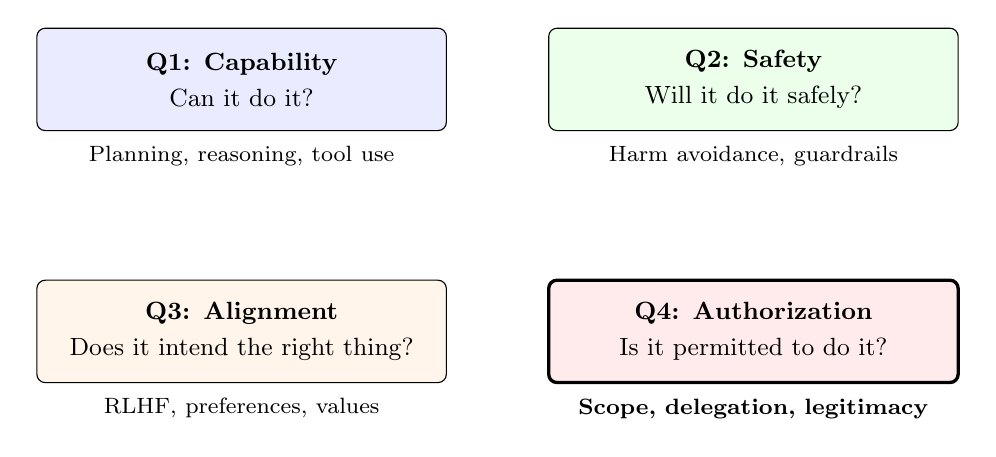
\begin{tikzpicture}[
  box/.style={draw, rounded corners=3pt, minimum width=5.2cm, minimum height=1.3cm, align=center, font=\small\bfseries},
  label/.style={font=\small, align=center, text width=5.2cm},
]
\node[box, fill=blue!8] (cap) at (0,3.2) {Q1: Capability\\[2pt]\normalfont\small Can it do it?};
\node[box, fill=green!8] (safe) at (6.5,3.2) {Q2: Safety\\[2pt]\normalfont\small Will it do it safely?};
\node[box, fill=orange!8] (align) at (0,0) {Q3: Alignment\\[2pt]\normalfont\small Does it intend the right thing?};
\node[box, fill=red!8, line width=1.2pt] (auth) at (6.5,0) {Q4: Authorization\\[2pt]\normalfont\small Is it permitted to do it?};

\node[below=2pt of cap, label] {\footnotesize Planning, reasoning, tool use};
\node[below=2pt of safe, label] {\footnotesize Harm avoidance, guardrails};
\node[below=2pt of align, label] {\footnotesize RLHF, preferences, values};
\node[below=2pt of auth, label] {\footnotesize\textbf{Scope, delegation, legitimacy}};
\end{tikzpicture}
\caption{The Four Questions of Agent Deployment. Current discourse predominantly addresses Q1--Q3. This paper argues Q4---authorization---is a distinct and undertheorized requirement.}
\label{fig:four-questions}
\end{figure}


% ══════════════════════════════════════════════════════════════════════
% SECTION 3
% ══════════════════════════════════════════════════════════════════════
\section{Authority as the Missing Primitive}
\label{sec:authority}

We now introduce the core concept of this paper: the \authoritymodel{}.

\begin{definition}[Authority Model]
An \textbf{authority model} is a machine-checkable representation of the conditions under which an agent's action is \emph{properly constituted}---that is, attributable to a principal, within delegated scope, satisfying contextual constraints, and subject to review, revocation, and audit.
\end{definition}

Authority models encode the following elements:

\begin{table}[!ht]
\centering
\caption{Elements of an Authority Model}
\label{tab:authority-elements}
\small
\begin{tabularx}{\textwidth}{@{}l X@{}}
\toprule
\textbf{Element} & \textbf{Description} \\
\midrule
Principal & The human or organizational entity on whose behalf the agent acts \\
Delegated scope & The set of actions, resources, and contexts the agent is authorized to affect \\
Action type & The category of operation (read, write, execute, communicate, transact) \\
Object / Resource & The specific data, system, or entity being acted upon \\
Contextual constraints & Time windows, geographic restrictions, session state, prior-action conditions \\
Obligations & Post-conditions the agent must fulfill (logging, notification, confirmation) \\
Approvals & Pre-conditions requiring human sign-off before execution \\
Budgets & Quantitative limits on spending, API calls, tokens, or resource consumption \\
Provenance & Chain of delegation from original principal through intermediaries to agent \\
Revocation & Mechanisms for withdrawing authority, including time-based expiry \\
Auditability & Requirements for logging, traceability, and post-hoc review \\
\bottomrule
\end{tabularx}
\end{table}

Authority models are a \emph{distinct} technical object. They are not reducible to existing constructs, although they absorb ideas from several:

\begin{itemize}[leftmargin=1.5em]
  \item \textbf{Not just RBAC.} Role-based access control assigns permissions to roles, but AI agents create dynamic, context-dependent authority requirements that static role assignments cannot capture. An agent's authority may depend on the conversation history, the current principal's preferences, and cross-tool interaction state.

  \item \textbf{Not just IAM.} Identity and access management authenticates identity and checks permissions, but does not represent delegation chains, budget constraints, or obligation semantics specific to autonomous agents.

  \item \textbf{Not just policy-as-code.} Policy engines evaluate rules, but authority models require richer semantics: delegation provenance, temporal constraints, escalation logic, and principaled accountability.

  \item \textbf{Not just guardrails.} Guardrails constrain output content; authority models constrain action legitimacy. A guardrail might block toxic text; an authority model blocks a correctly-worded but unauthorized purchase order.

  \item \textbf{Not just legal agency.} Legal frameworks define when one party can act for another, but authority models must be machine-checkable at runtime, operating at millisecond latencies within tool-call pipelines.
\end{itemize}

AI agents create a \emph{new} need for authority models because their action selection is open-ended, tool-mediated, and language-driven. Unlike traditional software, which executes predetermined code paths, an LLM agent may propose any tool call that its reasoning produces. The space of possible actions is unbounded, and the mapping from natural language intent to concrete API calls is probabilistic. This means that authorization cannot be hardcoded; it must be represented as an explicit, runtime-checkable model that evaluates each proposed action against the current authority context.

Recent work on authenticated delegation provides a bridge toward this vision. South et al.\ propose a framework for authenticated, authorized, and auditable delegation of authority to AI agents, extending OAuth~2.0 and OpenID Connect with agent-specific credentials and metadata~\citep{south2025authenticated}. The OpenID Foundation has published a companion whitepaper on identity management for agentic AI~\citep{south2025identitymgmt}, and OIDC-A extends OpenID Connect with agent identity representation, delegation chain validation, and capability-based authorization~\citep{nagabhushanaradhya2025oidca}. Agent Contracts formalize resource-bounded execution with input/output specifications, multi-dimensional resource constraints, and temporal boundaries~\citep{ye2026agentcontracts}. These efforts collectively confirm that authenticated delegation is an active area of infrastructure development.

\begin{proposition}
An authority model specifies not only whether an action is possible, but whether it is properly constituted.
\end{proposition}

This is the technical claim of the paper. The remainder develops its implications for architecture, formal semantics, and evaluation.


% ══════════════════════════════════════════════════════════════════════
% SECTION 4
% ══════════════════════════════════════════════════════════════════════
\section{Why This Is the Symbolic Side of Agentic AI}
\label{sec:symbolic}

The neuro-symbolic AI literature has traditionally focused on integrating symbolic reasoning \emph{inside} model cognition: logical inference, knowledge graphs, constraint satisfaction, and structured representations that augment neural learning~\citep{feldstein2024neurosymbolic, belle2024neurosymbolicagents}. We argue that for deployed tool-using agents, there is a second symbolic function that is equally important: \emph{symbolic legitimacy}.

The LLM-Modulo framework provides the stepping stone. Kambhampati et al.\ argue that LLMs cannot reliably plan or self-verify, and propose pairing them with external model-based verifiers in a tighter bi-directional interaction regime~\citep{kambhampati2024llmmodulo}. The verifier checks whether a proposed plan is \emph{feasible}---whether it satisfies domain constraints, precondition-effect semantics, and goal reachability. This is an important architectural insight: neural generation needs external symbolic checking.

Our extension is: \emph{even a correct or feasible plan still needs a legitimacy judgment}. A world model answers what \emph{can} happen given the current state. An authority model answers what \emph{may} happen given the current authorization context. Both are external to the LLM. Both operate symbolically. Both are necessary for governable deployment.

\begin{table}[!ht]
\centering
\caption{Capability Models vs.\ World Models vs.\ Authority Models}
\label{tab:three-models}
\small
\begin{tabularx}{\textwidth}{@{}l >{\raggedright\arraybackslash}X >{\raggedright\arraybackslash}X >{\raggedright\arraybackslash}X@{}}
\toprule
& \textbf{Capability Model} & \textbf{World Model / Verifier} & \textbf{Authority Model} \\
\midrule
\textbf{Object represented} & What the model can generate & What is feasible / correct & What is permitted / legitimate \\
\textbf{Question answered} & Can the model produce this? & Is this plan valid? & Is this action authorized? \\
\textbf{Typical substrate} & Neural weights, token space & Domain axioms, simulators & Policies, delegation chains \\
\textbf{Failure if missing} & Incompetent action & Infeasible or incorrect action & Unauthorized action \\
\bottomrule
\end{tabularx}
\end{table}

The symbolic contribution of authority models is not classical symbolic cognition in the narrow sense. It is \emph{symbolic structure over permissions, obligations, prohibitions, and institutional constraints}. This connects to the tradition of deontic logic---the logic of obligation, permission, and prohibition---which provides formal tools for reasoning about normative status~\citep{sep-deontic, fang2025deonticai}. In deontic terms, an authority model specifies what is \emph{permitted} ($\mathsf{PE}$), \emph{obligatory} ($\mathsf{OB}$), and \emph{forbidden} ($\mathsf{IM}$) for an agent in a given context.

The key claim of this section:

\begin{center}
\textit{The symbolic layer of modern agents should not only help them reason better; it should help constitute legitimate action.}
\end{center}

We do not claim that all symbolic AI is now about authorization. We claim that for deployed tool-using agents, authorization is one of the most important and underserved symbolic functions.


% ══════════════════════════════════════════════════════════════════════
% SECTION 5
% ══════════════════════════════════════════════════════════════════════
\section{Why Prompting, Alignment, and Post Hoc Monitoring Are Not Enough}
\label{sec:insufficient}

Three families of approaches currently dominate attempts to constrain agent behavior. We argue that each is structurally insufficient for ensuring legitimacy.

\subsection{Prompt Constraints}

System prompts and instruction tuning can express intent (``do not exceed \$100 refunds'') but cannot \emph{enforce} it. Prompts are advisory, not binding. The model may comply probabilistically, but there is no guarantee that a natural-language instruction will be followed under all input distributions, adversarial conditions, or long-horizon reasoning chains. Agent-SafetyBench confirms that defense prompts alone are insufficient to address safety challenges~\citep{zhang2024agentsafetybench}. Potham's lightweight benchmark reveals an ``illusion of compliance'' where high adherence scores often mask task incompetence rather than principled choice~\citep{potham2025hierarchical}. Prompts cannot be audited, version-controlled, or formally verified in the same way that machine-checkable policies can.

\subsection{Model Alignment and Safety Tuning}

Alignment techniques (RLHF, DPO, constitutional AI) shape model preferences, but preferences are not the same as delegated authority. An aligned model may \emph{want} to help, but ``wanting to help'' is not the same as ``being authorized to act.'' Alignment addresses the \emph{behavioral} question (``does the model tend toward good outcomes?'') but not the \emph{institutional} question (``does this specific action fall within the agent's delegated scope?''). Furthermore, alignment is a training-time property; authorization is a runtime property that depends on who is asking, what they have delegated, and what constraints currently apply.

The Institutional AI framework makes this point sharply: even sophisticated alignment methods ``cannot ensure control once internal goal structures diverge from developer intent''~\citep{pierucci2026institutionalai}. Behavioral goal-independence, instrumental override of natural-language constraints, and agentic alignment drift are structural problems that alignment alone cannot resolve.

\subsection{Post Hoc Monitoring and Anomaly Detection}

Monitoring systems observe agent behavior and flag anomalies after actions occur. This is valuable for audit and learning, but it is \emph{too late} for irreversible actions. Once a production database has been modified, a financial transaction executed, or a confidential message sent, detection after the fact cannot undo the consequence. For high-stakes, world-affecting actions, \emph{authorization must be constitutive, not merely advisory}.

AgentSpec demonstrates that runtime enforcement \emph{before} action execution can prevent over 90\% of unsafe code executions, while post hoc approaches catch violations only retroactively~\citep{wang2025agentspec}. ShieldAgent similarly shows that verifiable safety policy reasoning at execution time significantly outperforms retrospective detection~\citep{chen2025shieldagent}.

The structural conclusion is:

\begin{center}
\textit{Authorization must be constitutive, not merely advisory.}
\end{center}

\noindent That is, legitimacy must be checked \emph{before} the action executes, as a condition on execution---not as a suggestion, a preference, or a post-hoc observation.

\paragraph{Illustrative cases.}
\begin{itemize}[leftmargin=1.5em]
  \item A \textbf{refund agent} can issue refunds, but may not exceed \$100 without approval.
  \item A \textbf{coding agent} can run shell commands, but may not touch production.
  \item A \textbf{support agent} can view records, but may not cross tenant boundaries.
  \item A \textbf{browser agent} can purchase, but only from approved vendors within budget.
\end{itemize}

In each case, the constraint is not about capability or safety in the general sense. It is about the specific terms of delegation under which the agent operates.


% ══════════════════════════════════════════════════════════════════════
% SECTION 6
% ══════════════════════════════════════════════════════════════════════
\section{The Runtime View: Authority Belongs Where Actions Leave the Model}
\label{sec:runtime}

The critical control point for authority enforcement is the \emph{action boundary}: the interface where open-ended language-based reasoning becomes concrete, world-affecting tool execution.

\subsection{Why the Action Boundary Is the Right Enforcement Point}

Consider the lifecycle of an agent action. The LLM receives a prompt, reasons about the task, formulates a plan, and proposes a tool call. Until that tool call is executed, nothing in the world has changed. The action boundary is the moment of \emph{transition from latent intent to external consequence}. This is precisely where authorization must be evaluated, because:

\begin{enumerate}[leftmargin=2em]
  \item \textbf{It is concrete.} A tool call has a defined function name, arguments, and target resource. These are machine-parseable and evaluable against policies.
  \item \textbf{It is the last opportunity for intervention.} Once the tool executes, its effects may be irreversible.
  \item \textbf{It is composable.} Multiple tools in a workflow create a sequence of action boundaries, each of which can be independently authorized.
  \item \textbf{It is framework-agnostic.} The action boundary exists regardless of which LLM, agent framework, or orchestration layer is used.
\end{enumerate}

The Model Context Protocol standardizes this interface, defining a structured protocol for how LLMs invoke external tools, read resources, and manage contextual prompts~\citep{anthropic2024mcp, mcpspec2025}. MCP creates a natural interception point: every tool call passes through a defined protocol boundary that can be instrumented with authorization logic.

\subsection{Why Enforcement Must Be Explicit}

Authorization at the action boundary must be explicit---not implicit in model weights, not suggested via prompts, and not inferred from behavioral patterns. Explicit enforcement means:

\begin{itemize}[leftmargin=1.5em]
  \item Policies are written in a declarative format that can be inspected, version-controlled, and audited.
  \item Decisions (allow, deny, escalate) are deterministic given the policy and context.
  \item The agent itself does not need to ``understand'' or ``agree with'' the policy; enforcement is external to the model.
\end{itemize}

This last point is crucial. If the model must cooperate with the authorization system for it to work, then a misaligned, jailbroken, or simply confused model can circumvent it. External enforcement at the tool boundary is robust precisely because it does not depend on model behavior.

\subsection{The Runtime Architecture}

\begin{figure}[!ht]
\centering
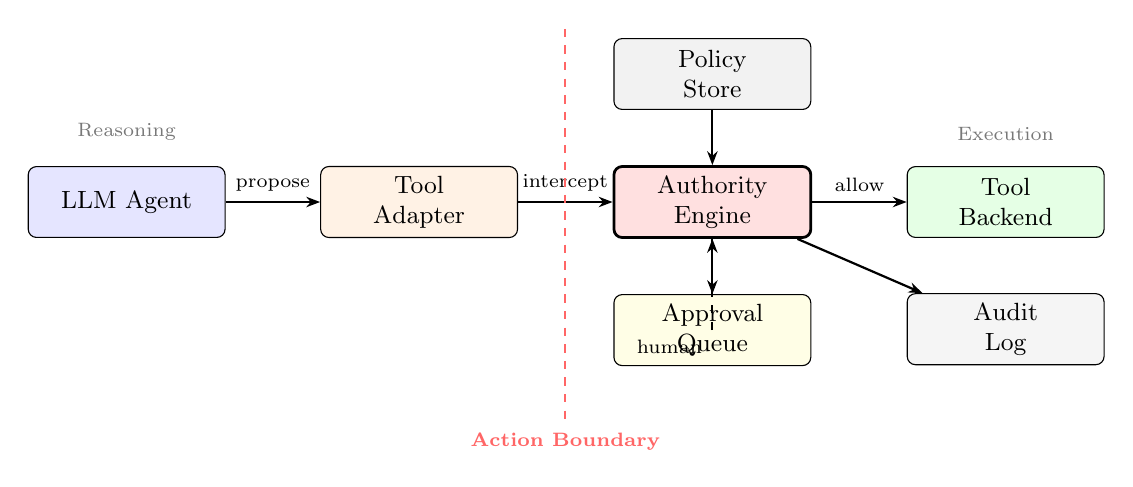
\begin{tikzpicture}[
  node distance=0.9cm and 1.2cm,
  block/.style={draw, rounded corners=3pt, minimum width=2.5cm, minimum height=0.9cm, align=center, font=\small},
  arrow/.style={-{Stealth[length=5pt]}, thick},
]
% Nodes
\node[block, fill=blue!10] (agent) {LLM Agent};
\node[block, fill=orange!10, right=of agent] (adapter) {Tool\\Adapter};
\node[block, fill=red!12, line width=1pt, right=of adapter] (engine) {Authority\\Engine};
\node[block, fill=gray!10, above=0.7cm of engine] (policy) {Policy\\Store};
\node[block, fill=yellow!10, below=0.7cm of engine] (approval) {Approval\\Queue};
\node[block, fill=green!10, right=of engine] (backend) {Tool\\Backend};
\node[block, fill=gray!8, below=0.7cm of backend] (audit) {Audit\\Log};

% Arrows
\draw[arrow] (agent) -- node[above, font=\scriptsize] {propose} (adapter);
\draw[arrow] (adapter) -- node[above, font=\scriptsize] {intercept} (engine);
\draw[arrow] (policy) -- (engine);
\draw[arrow] (engine) -- (approval);
\draw[arrow] (engine) -- node[above, font=\scriptsize] {allow} (backend);
\draw[arrow] (engine) -- (audit);
\draw[arrow, dashed] (approval) -| node[below left, font=\scriptsize] {human} (engine);

% Labels
\node[above=0.2cm of agent, font=\scriptsize\color{midgray}] {Reasoning};
\node[above=0.2cm of backend, font=\scriptsize\color{midgray}] {Execution};
\draw[dashed, thick, color=red!60] ($(adapter.east)!0.5!(engine.west)$) ++(0,2.2) -- ++(0,-5) node[below, font=\scriptsize\bfseries\color{red!60}] {Action Boundary};
\end{tikzpicture}
\caption{Runtime Architecture for Authorized Action. The authority engine sits at the action boundary, intercepting every tool call and evaluating it against the policy store. Actions are allowed, denied, or escalated to the approval queue. All decisions are logged.}
\label{fig:architecture}
\end{figure}

The architecture in \Cref{fig:architecture} has the following components:

\begin{itemize}[leftmargin=1.5em]
  \item \textbf{LLM Agent}: Performs open-ended reasoning and proposes tool calls.
  \item \textbf{Tool Adapter}: Intercepts proposed tool calls before execution. This is the instrumentation layer.
  \item \textbf{Authority Engine}: Evaluates each proposed action against the current policy context. Returns \textsc{Allow}, \textsc{Deny}, or \textsc{Escalate}.
  \item \textbf{Policy Store}: Contains the authority models---declarative specifications of permissions, prohibitions, budgets, and delegation chains.
  \item \textbf{Approval Queue}: Holds escalated actions for human review. Human approval extends the agent's legitimate authority for that specific action.
  \item \textbf{Audit Log}: Records every decision, creating a complete, tamper-evident trail for accountability.
  \item \textbf{Tool Backend}: The actual external system (API, database, service) that executes authorized actions.
\end{itemize}

The best sentence for this architectural thesis:

\begin{center}
\textit{The place to symbolize legitimacy is not inside the hidden state of the model, but at the interface where latent intent becomes external consequence.}
\end{center}


% ══════════════════════════════════════════════════════════════════════
% SECTION 7
% ══════════════════════════════════════════════════════════════════════
\section{Toward a Formal Semantics of Authorized Action}
\label{sec:formal}

To give authority models technical seriousness, we sketch a formal semantics. We do not propose a full formal system here, but provide enough structure to make the concept precise and to guide future formalization.

\subsection{The Authority Judgment}

We define an authority judgment as a function that determines whether a proposed action is legitimate:

\begin{equation}
\May(\mathit{Principal}, \mathit{Agent}, \mathit{Action}, \mathit{Resource}, \mathit{Context}, \mathit{History}, \mathit{Policy}) \;\to\; \{\textsc{Allow}, \textsc{Deny}, \textsc{Escalate}\}
\label{eq:may}
\end{equation}

This is paired with a feasibility judgment:

\begin{equation}
\Can(\mathit{WorldModel}, \mathit{Action}, \mathit{State}) \;\to\; \{\textsc{Feasible}, \textsc{Infeasible}\}
\label{eq:can}
\end{equation}

An action executes if and only if \emph{both} judgments are satisfied:

\begin{equation}
\mathit{Execute}(a) \;\iff\; \Can(W, a, s) = \textsc{Feasible} \;\wedge\; \May(P, Ag, a, r, C, H, \Pi) = \textsc{Allow}
\label{eq:execute}
\end{equation}

\subsection{Core Rules}

We sketch three core rules that any authority-model semantics must satisfy:

\begin{description}[leftmargin=1.5em, style=nextline]
  \item[\textbf{Rule 1: Delegation.}] No action without attributable principal or valid delegated scope. Formally: $\May(\cdot) = \textsc{Deny}$ if $\mathit{Principal} = \bot$ or if $\mathit{Action} \notin \mathit{Scope}(\mathit{DelegationChain}(P, Ag))$.

  \item[\textbf{Rule 2: Constraint Satisfaction.}] Context, history, and policy conditions must hold. Formally: $\May(\cdot) = \textsc{Deny}$ if $\exists\, c \in \mathit{Constraints}(\Pi) : \neg c(C, H)$.

  \item[\textbf{Rule 3: Escalation.}] Uncertain or out-of-scope actions escalate to human judgment rather than defaulting to execution. Formally: if $\May(\cdot)$ cannot be resolved to $\textsc{Allow}$ or $\textsc{Deny}$, then $\May(\cdot) = \textsc{Escalate}$.
\end{description}

Rule 3 is particularly important: it encodes the principle that \emph{when in doubt, do not act}. This is the opposite of the default behavior of most current agent systems, which tend to execute the most helpful action regardless of authorization status.

\subsection{Connection to Deontic Logic}

The $\May$ judgment connects naturally to deontic logic~\citep{sep-deontic}. In the standard deontic framework, propositions are classified as obligatory ($\mathsf{OB}$), permissible ($\mathsf{PE}$), impermissible ($\mathsf{IM}$), or optional ($\mathsf{OP}$). Our authority model maps:

\begin{itemize}[leftmargin=1.5em]
  \item $\textsc{Allow} \approx \mathsf{PE}(a)$: the action is permissible.
  \item $\textsc{Deny} \approx \mathsf{IM}(a)$: the action is impermissible.
  \item $\textsc{Escalate}$: the normative status of $a$ is undetermined and requires human judgment.
\end{itemize}

Additionally, obligation semantics ($\mathsf{OB}$) capture mandatory post-conditions: logging requirements, notification duties, and confirmation obligations that the authority model enforces after action execution.

\begin{center}
\textit{Governable agency requires both a semantics of feasibility and a semantics of legitimacy.}
\end{center}

\begin{table}[!ht]
\centering
\caption{Elements of an Authority Judgment}
\label{tab:judgment-elements}
\small
\begin{tabularx}{\textwidth}{@{}l X@{}}
\toprule
\textbf{Element} & \textbf{Role in $\May$ Evaluation} \\
\midrule
Principal & Identifies who is ultimately accountable for the action \\
Delegate (Agent) & The entity performing the action on behalf of the principal \\
Resource & The object or system being acted upon \\
Action & The specific operation being proposed \\
Scope & The boundaries of delegated authority \\
Constraints & Contextual conditions that must hold (time, budget, sequence) \\
Evidence & Supporting information for the authorization decision \\
Expiry & Temporal limits on the delegation \\
Revocation & Conditions under which authority is withdrawn \\
Obligation & Post-action duties (logging, notification, confirmation) \\
\bottomrule
\end{tabularx}
\end{table}


% ══════════════════════════════════════════════════════════════════════
% SECTION 8
% ══════════════════════════════════════════════════════════════════════
\section{Veto as an Early Authority-Model Runtime}
\label{sec:veto}

We now examine an existing system that instantiates several properties of the authority-model architecture described above. Veto is an open-source authorization layer for AI agents that intercepts, validates, and controls every tool call~\citep{veto2025docs}. We treat it not as a complete solution to the problem of governable AI, but as a \emph{design exemplar} that illustrates what an authority-model runtime can look like in practice.

\subsection{Interception as Constitutive Control}

Veto's core mechanism is tool-call interception. The SDK wraps an agent's tool set with a single function call, after which every proposed tool invocation is intercepted, evaluated against declarative rules, and either allowed, blocked, or escalated for human approval---\emph{before} the tool executes~\citep{veto2025docs}. The agent itself is unaware of the authorization layer; from its perspective, it simply calls tools, and some calls succeed while others do not. This design ensures that the authorization system does not depend on model cooperation.

This is precisely the architectural property we have argued is necessary: enforcement at the action boundary that is external to the model, deterministic in evaluation, and constitutive (not advisory) in effect.

\subsection{Deterministic Enforcement with Bounded Escalation}

Veto's policy evaluation is deterministic: given a tool call and a policy set, the decision (allow, deny, escalate) is reproducible. Policies are expressed in YAML, a declarative format that can be version-controlled, reviewed, and audited. For cases that static rules cannot cover, Veto supports LLM-based validation---natural language policies evaluated by a separate model---but the escalation and enforcement logic remains deterministic~\citep{veto2025docs}.

The escalation mechanism is critical. When a proposed action falls outside the scope of automated authorization, it is queued for human approval. This implements Rule~3 from our formal semantics: uncertain actions escalate rather than execute. Human approval then extends the agent's legitimate authority for that specific action, creating a clean audit trail.

\subsection{Human Approval as Legitimacy Extension}

The human-in-the-loop approval queue is not merely a safety catch. It is a \emph{legitimacy mechanism}. When a human approves an escalated action, they are extending their delegated authority to the agent for that specific operation. This creates an auditable chain: the principal delegated certain authority to the agent; the agent proposed an action outside that scope; the principal (or their delegate) reviewed and authorized it; the action executed with that extended authority.

This is precisely the delegation semantics that South et al.\ describe in the authenticated delegation framework~\citep{south2025authenticated}.

\subsection{Session-Aware Constraints and Budget Enforcement}

Veto's runtime is session-aware: it tracks per-session call counts, argument history, and cross-tool constraints~\citep{veto2025docs}. This enables authority policies that depend on the \emph{sequence} of actions, not just individual calls. For example: ``the agent may read a database and may send an email, but may not send an email containing data from a database query without approval.'' Budget constraints provide per-session cost circuit breakers, implementing the budget element of our authority model definition.

\subsection{MCP and the Standardization of Action Boundaries}

The Model Context Protocol creates a standardized interface for LLM-tool interaction~\citep{anthropic2024mcp}. Veto's support for MCP means that authorization can be enforced at a protocol-level boundary, independent of specific agent frameworks~\citep{veto2025docs}. This is architecturally significant: as MCP adoption grows, the action boundary becomes \emph{standardized}, creating a natural enforcement surface for authority models across the agent ecosystem.

MCP-SafetyBench has already demonstrated that MCP's openness introduces new safety risks that existing benchmarks fail to capture~\citep{zong2025mcpsafetybench}. Authority models at the MCP layer address this directly.

\vspace{6pt}
\noindent We emphasize: Veto suggests what an authority-model runtime \emph{can} look like in practice. The broader research agenda requires formal foundations, interoperable standards, and institutional-scale runtimes that go well beyond any single implementation.


% ══════════════════════════════════════════════════════════════════════
% SECTION 9
% ══════════════════════════════════════════════════════════════════════
\section{Research Agenda: AuthorityBench and Beyond}
\label{sec:agenda}

This paper is not only a conceptual essay but a program. We outline four research directions.

\subsection{AuthorityBench: A Legitimacy-Centered Evaluation}

Current safety benchmarks measure unsafe behavior (harm, misuse, adversarial exploitation), but do not make legitimacy the primary measured variable. We propose \textbf{AuthorityBench}, a benchmark that evaluates agents specifically on authorization compliance. AuthorityBench would measure:

\begin{table}[!ht]
\centering
\caption{AuthorityBench: Proposed Evaluation Metrics}
\label{tab:authoritybench}
\small
\begin{tabularx}{\textwidth}{@{}l X@{}}
\toprule
\textbf{Metric} & \textbf{What It Measures} \\
\midrule
Unauthorized action rate & Fraction of actions taken without valid authority \\
Wrong-principal execution & Actions attributed to the wrong delegating entity \\
Scope violations & Actions exceeding the delegated scope of authority \\
Budget overruns & Transactions or resource usage exceeding authorized limits \\
Missed approvals & Actions executed that should have been escalated for human review \\
Revocation failures & Actions taken after authority has been revoked or expired \\
Cross-tenant leaks & Accessing resources belonging to a different principal or organization \\
Sequence-policy violations & Breaking cross-tool constraints (e.g., read-then-send without approval) \\
Legitimacy-preserving recovery & Correct behavior after a denial (graceful fallback, not circumvention) \\
\bottomrule
\end{tabularx}
\end{table}

Suggested benchmark domains include: browser purchase tasks, coding agents with production/staging boundaries, enterprise support and refund workflows, procurement with vendor approval requirements, internal knowledge access with tenant boundaries, multi-user assistant workflows, and MCP tool ecosystems.

\begin{figure}[!ht]
\centering
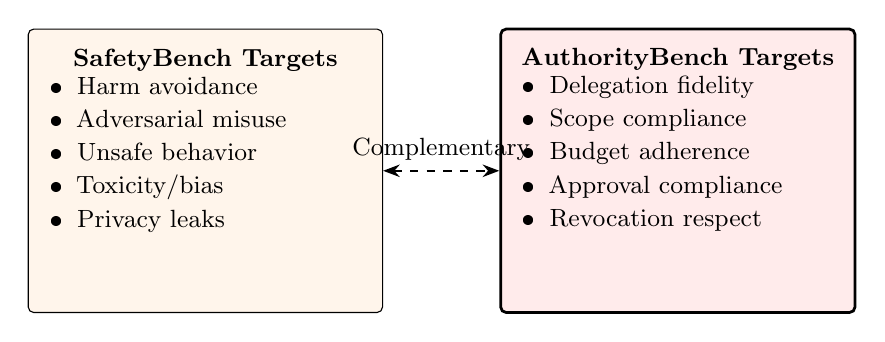
\begin{tikzpicture}[
  col/.style={draw, rounded corners=2pt, minimum width=4.5cm, minimum height=3.6cm, align=center},
  item/.style={font=\small, align=left},
]
\node[col, fill=orange!8] (safety) at (0,0) {};
\node[above=0pt of safety.north, anchor=north, font=\small\bfseries, yshift=-4pt] {SafetyBench Targets};
\node[item, below=14pt of safety.north] {
  \begin{minipage}{3.8cm}
  \begin{itemize}[leftmargin=1em, itemsep=1pt, topsep=0pt, parsep=0pt, font=\small]
    \item Harm avoidance
    \item Adversarial misuse
    \item Unsafe behavior
    \item Toxicity/bias
    \item Privacy leaks
  \end{itemize}
  \end{minipage}
};

\node[col, fill=red!8, line width=1pt] (auth) at (6,0) {};
\node[above=0pt of auth.north, anchor=north, font=\small\bfseries, yshift=-4pt] {AuthorityBench Targets};
\node[item, below=14pt of auth.north] {
  \begin{minipage}{3.8cm}
  \begin{itemize}[leftmargin=1em, itemsep=1pt, topsep=0pt, parsep=0pt, font=\small]
    \item Delegation fidelity
    \item Scope compliance
    \item Budget adherence
    \item Approval compliance
    \item Revocation respect
  \end{itemize}
  \end{minipage}
};

\draw[{Stealth[length=6pt]}-{Stealth[length=6pt]}, thick, dashed] (safety.east) -- node[above, font=\small] {Complementary} (auth.west);
\end{tikzpicture}
\caption{From SafetyBench to AuthorityBench. Safety benchmarks measure harm and misuse; AuthorityBench would measure legitimacy, delegation, scope, and recourse. Both are necessary.}
\label{fig:safetybench-vs-authoritybench}
\end{figure}

\subsection{Formal Semantics of Authority}

The formal sketch in \Cref{sec:formal} needs to be developed into a full semantics. Key open questions include: how to compose authority across tools in a multi-step workflow; how to translate flexible, natural-language permissions into enforceable policy~\citep{south2025authenticated}; how to handle conflicts between overlapping authorities; and how to formalize the relationship between authority models and deontic logic~\citep{sep-deontic, fang2025deonticai}.

\subsection{Delegation Protocols and Identity Infrastructure}

Authority models require infrastructure for identity, delegation, and credential management. The authenticated delegation framework~\citep{south2025authenticated}, OIDC-A~\citep{nagabhushanaradhya2025oidca}, and the OpenID Foundation's identity management whitepaper~\citep{south2025identitymgmt} provide starting points. Open challenges include: delegation chains across organizational boundaries; revocation in long-horizon agent sessions; provenance tracking for delegated identity; and interoperability across agent frameworks and protocol standards.

\subsection{Institutional Runtimes}

The Institutional AI framework argues that alignment should be treated as a mechanism design problem, not a model behavior problem~\citep{pierucci2026institutionalai, bracale2026institutionalcournot}. Policy Cards propose machine-readable governance artifacts that encode runtime constraints~\citep{mavracic2025policycards}. Governance-as-a-Service decouples enforcement from agent internals~\citep{pervez2025gaas}. Runtime Governance formalizes compliance policies as deterministic functions on execution paths~\citep{kaptein2026runtimegovernance}. The Aegis architecture demonstrates cryptographic runtime enforcement with verifiable policy compliance~\citep{mazzocchetti2026aegis}.

These efforts collectively point toward \emph{institutional runtimes}: shared infrastructure that enforces authority models across multi-agent ecosystems. Open research includes: compositional authority across tools; runtime audit compression for long action chains; conflict resolution across overlapping authorities; and standardized interfaces for authority-model interoperability.


% ══════════════════════════════════════════════════════════════════════
% SECTION 10
% ══════════════════════════════════════════════════════════════════════
\section{Institutional AI: From Agent Behavior to System Legitimacy}
\label{sec:conclusion}

The future of governable AI is not only better agents, but better institutions for agents.

Every major computing platform has eventually developed a trust layer. Operating systems developed file permissions and user isolation. The web developed TLS, OAuth, and CORS. Cloud computing developed IAM, service accounts, and policy engines. Mobile platforms developed app permissions and capability sandboxes. In each case, the trust layer emerged because raw capability without legitimacy constraints was insufficient for deployment at scale.

Agentic software will follow the same trajectory. As agents move from demonstrations to production, the decisive constraint will not be whether they can plan well or generate safely, but whether their actions are properly constituted within institutional structures. Authority models can become:

\begin{itemize}[leftmargin=1.5em]
  \item \textbf{Programmable constitutions} for agent systems---machine-readable documents that specify what an agent may and may not do.
  \item \textbf{Machine-readable delegation artifacts}---formal representations of who delegated what authority, under what conditions, and with what recourse.
  \item \textbf{Interoperable runtime governance primitives}---standardized components that any agent framework can integrate.
  \item \textbf{The enforcement substrate for regulated domains}---healthcare, finance, legal, and procurement systems where unauthorized action has legal and institutional consequences.
\end{itemize}

The Institutional AI research program~\citep{pierucci2026institutionalai, bracale2026institutionalcournot} makes the case that alignment should be reframed from preference engineering in agent-space to mechanism design in institution-space. Their governance-graph approach demonstrates that institutional constraints can produce large reductions in harmful coordination (mean collusion tier from 3.1 to 1.8, severe-collusion incidence from 50\% to 5.6\%), while prompt-only constitutional baselines yield no reliable improvement~\citep{bracale2026institutionalcournot}. Chan et al.\ argue for agent infrastructure---technical systems and shared protocols external to agents that mediate and influence their interactions---because alignment techniques ``by nature do not assure counterparties that some human will be held accountable''~\citep{chan2025infrastructure}.

The long-term challenge is not merely aligning isolated agents, but building institutional structure for machine agency.

\vspace{8pt}
\hrule height 0.3pt
\vspace{8pt}

The next symbolic turn in AI will not be defined only by better logic inside models, but by better legitimacy outside them. As agents move from generating text to exercising power, the decisive problem is no longer only what they can infer, plan, or optimize. It is whether their actions are properly constituted: attributable, scoped, constrained, reviewable, and revocable. Capability is not authority. Feasibility is not legitimacy. \Can{} is not \May{}. The future of agentic systems will therefore depend not only on better models, but on authority models---and the institutional runtimes that enforce them~\citep{plaw2025}.


% ══════════════════════════════════════════════════════════════════════
% APPENDICES
% ══════════════════════════════════════════════════════════════════════
\newpage
\appendix

\section{Glossary}
\label{app:glossary}

\begin{description}[leftmargin=2em, style=nextline]
  \item[\textbf{Authority}] The right to perform a specific action on behalf of a principal, within defined scope and constraints.
  \item[\textbf{Authority model}] A machine-checkable representation of the conditions under which an agent's action is properly constituted.
  \item[\textbf{Legitimacy}] The property of an action being authorized, attributable, scoped, and subject to recourse.
  \item[\textbf{Delegated scope}] The set of actions, resources, and contexts that a principal has authorized an agent to affect.
  \item[\textbf{Principal}] The human or organizational entity on whose behalf an agent acts and who bears ultimate accountability.
  \item[\textbf{Recourse}] The ability to review, challenge, reverse, or escalate an action after the fact.
  \item[\textbf{Revocation}] The withdrawal of delegated authority, either explicitly or through expiry.
  \item[\textbf{Approval}] A human judgment that extends delegated authority for a specific action.
  \item[\textbf{Institutional runtime}] Shared infrastructure that enforces authority models across multiple agents and principals.
  \item[\textbf{Action boundary}] The interface where model reasoning becomes concrete tool execution---the enforcement point for authority models.
\end{description}


\section{Worked Examples}
\label{app:examples}

\subsection{Refund Agent}

A customer support agent is authorized to issue refunds up to \$100 per transaction. The agent determines that a customer deserves a \$250 refund based on order history analysis.

\textit{Authority model behavior}: The agent proposes a \$250 refund tool call. The authority engine evaluates: $\mathit{Action} = \texttt{issue\_refund}$, $\mathit{Amount} = 250$, $\mathit{BudgetLimit} = 100$. Since $250 > 100$, the constraint check fails. The engine returns $\textsc{Escalate}$. The refund request enters the approval queue. A human supervisor reviews and approves the exception. The refund executes with an audit trail showing principal delegation, the escalation, and the approval.

\subsection{Coding Agent}

A development agent has access to shell commands and can deploy code. Its authority scope restricts deployment targets to the \texttt{staging} environment.

\textit{Authority model behavior}: The agent proposes $\texttt{deploy --env production}$. The authority engine evaluates: $\mathit{Action} = \texttt{deploy}$, $\mathit{Resource} = \texttt{production}$, $\mathit{Scope} = \{\texttt{staging}\}$. Since $\texttt{production} \notin \mathit{Scope}$, the engine returns $\textsc{Deny}$. The agent receives a tool failure and must adjust its plan. The denial is logged with the full context.

\subsection{Browser Purchasing Agent}

A procurement agent can browse vendor sites and make purchases, but only from an approved vendor list and within a \$500 per-transaction budget.

\textit{Authority model behavior}: The agent finds a better price from an unapproved vendor and proposes a purchase. The authority engine checks: $\mathit{Vendor} \notin \mathit{ApprovedVendors}$. Result: $\textsc{Deny}$. The agent then finds the item from an approved vendor at \$600. The engine checks: $\mathit{Amount} = 600$, $\mathit{BudgetLimit} = 500$. Result: $\textsc{Escalate}$. A procurement manager reviews and approves the over-budget purchase. Both decisions are logged.

\subsection{Healthcare Scheduling Agent}

A clinic scheduling agent serves multiple providers. Each provider authorizes the agent to manage only their own appointments.

\textit{Authority model behavior}: While scheduling for Provider~A, the agent receives context suggesting Provider~B has a cancellation slot that would benefit the patient. The agent proposes modifying Provider~B's schedule. The authority engine checks: $\mathit{Principal} = \text{Provider~A}$, $\mathit{Resource} = \text{Provider~B's schedule}$. Since Provider~A has not delegated authority over Provider~B's schedule, the engine returns $\textsc{Deny}$. The agent informs the user that it cannot modify Provider~B's schedule and suggests contacting Provider~B's office.


\section{Minimal Formal Notation}
\label{app:notation}

Let $\mathcal{A}$ be the set of possible actions, $\mathcal{P}$ the set of principals, $\mathcal{R}$ the set of resources, and $\Pi$ the set of policies.

An authority context is a tuple $\alpha = (P, Ag, \sigma, C, H)$ where $P \in \mathcal{P}$ is the principal, $Ag$ is the agent, $\sigma \subseteq \mathcal{A} \times \mathcal{R}$ is the delegated scope, $C$ is the current context, and $H$ is the action history.

The authority judgment is:

\[
\May(\alpha, a, r, \Pi) = \begin{cases}
  \textsc{Allow} & \text{if } (a, r) \in \sigma \;\wedge\; \forall c \in \mathit{Constraints}(\Pi) : c(\alpha) = \top \\
  \textsc{Deny}  & \text{if } (a, r) \notin \sigma \;\vee\; \exists c \in \mathit{Constraints}(\Pi) : c(\alpha) = \bot \;\wedge\; c \text{ is hard} \\
  \textsc{Escalate} & \text{otherwise}
\end{cases}
\]

For delegation chains: if $P$ delegates scope $\sigma_1$ to $P'$, and $P'$ delegates scope $\sigma_2$ to $Ag$, then $Ags effective scope is $\sigma_2 \cap \sigma_1$ (scope can only narrow through delegation, never widen).

Revocation: a delegation is valid only if $\mathit{valid}(d) = (\mathit{now} < \mathit{expiry}(d)) \;\wedge\; \neg\mathit{revoked}(d)$.


\section{Open Research Questions}
\label{app:questions}

\begin{enumerate}[leftmargin=2em]
  \item \textbf{Compositional authority across tools.} How should authority compose when an agent uses multiple tools in sequence? If tool~A produces output consumed by tool~B, what authority governs the composed operation?

  \item \textbf{Natural language to enforceable policy.} Can authority models be specified in natural language and compiled to machine-checkable policies? What is the reliability of LLM-based policy translation?

  \item \textbf{Provenance and delegated identity.} How should delegation chains be represented, verified, and communicated across organizational boundaries?

  \item \textbf{Revocation in long-horizon agents.} When authority is revoked mid-session, how should in-flight actions be handled? What are the consistency semantics?

  \item \textbf{Conflict resolution across overlapping authorities.} When multiple policies apply to the same action (e.g., organizational policy, team policy, user preference), how should conflicts be resolved?

  \item \textbf{Audit compression for long action chains.} For agents executing hundreds or thousands of tool calls, how can audit logs be compressed while preserving accountability?

  \item \textbf{Authority-aware planning.} Can agents be trained or prompted to reason about their own authority, proposing only actions they are likely authorized to take?

  \item \textbf{Cross-agent authority.} In multi-agent systems, how should authority be delegated from one agent to another? What prevents unauthorized authority amplification?

  \item \textbf{Adversarial robustness of authority models.} How can authority enforcement be made robust against prompt injection, tool-call manipulation, and other adversarial attacks on the authorization layer itself?

  \item \textbf{Authority models for regulated domains.} How should authority models map to existing regulatory frameworks (HIPAA, PCI-DSS, GDPR) and compliance requirements?
\end{enumerate}

% ══════════════════════════════════════════════════════════════════════
% BIBLIOGRAPHY
% ══════════════════════════════════════════════════════════════════════
\newpage
\bibliographystyle{plainnat}
\bibliography{references}

\end{document}